
%Rodzia� 7
\newpage
\chapter{Sterowanie optymalne i sterowanie odporne - Kuba}
  \section{Sterowanie o zmiennej strukturze mechanizm�w wielocz�onowych}
  
  \subsection{Wst?p do sterowania ?lizgowego}
  Niech $s(x)$ b?dzie funkcj?, nazywan? funkcj? prze??czaj?c?, opisan? zale?no?ci?:
  %
 \begin{equation}
 	s(x)=Hx(t)
 \end{equation}
  %
  gdzie: $H\in R^{m\times n}$ i jest pe?nego rz?du, $n$ - liczba zmiennych stanu uk?adu, $m$ - liczba sygna?�w steruj?cych.
  
  Niech zbi�r punkt�w w przestrzeni zmiennych stanu $\Psi$ b?dzie opisany jako:
  %
	\begin{equation}
	\Psi=\left\{x\in R^{n}:s(x)=0\right\}
	\end{equation}
  %
  Zbi�r  $\Psi$ nazywany jest powierzchni? ?lizgow?. Mo?na go te? nazwa? hiperpowierzchni?, lub quasipowierzchni? ?lizgow?, gdy? wymiar $\Psi$ zale?y od liczby  zmiennych stanu i liczby wej?? steruj?cych zgodnie z zale?no?ci?:
   %
  \begin{equation}
  n_{\Psi}=n-m
  \end{equation}
  %
  Przyk?adowo dla dw�ch zmiennych stanu i jednego wej?cia steruj?cego zbi�r $\Psi$ jest  krzyw? o wymiarze 1, dla uk?adu o trzech zmiennych stanu i jednym wej?ciu steruj?cym jest p?aszczyzn?, dla uk?adu o sze?ciu zmiennych stanu i dw�ch wej?ciach steruj?cych ma wymiar $n_{\Psi}=4$
  
  Przyjmuj?c, za \cite{hung:1993}:
  %
  \begin{equation}
  s(x)=[s_{1}(x),\dots,s_{m}(x)]^{T}, H=[H_{1},\dots,H_{m}] 
  \end{equation}
  %
  gdzie: $H_{i}=[h_{i1}\quad h_{i2} \dots h_{in}], i=1,\dots,m$   r�wnanie (4.5) mo?na przedstawi? w postaci $i$ r�wna?:
   %
 	\begin{equation}
 	s_{i}(x)=H_{i}x\quad \text{gdzie} i=1,\dots,m 
 	\end{equation}
  %
  Zbi�r punkt�w $\Psi_{i}=\left\{x\in R^{n}:s_{i}(x) = 0\right\} $ opisuje powierzchni? $\Psi_{i}$ zwan? $i$-t? sk?adow? powierzchni? ?lizgow?.

  Metoda sterowania ?lizgowego polega na odpowiednim generowaniu sygna?u steruj?cego zale?nego od po?o?enia uk?adu w przestrzeni zmiennych stanu wzgl?dem powierzchni ?lizgowej $\Psi$. Uk?ad ze sterowaniem ?lizgowym jest tak zaprojektowany, aby jego trajektoria kierowa?a si? zawsze w stron? powierzchni ?lizgowej ?. W momencie gdy  stan uk?adu j? osi?gnie, zaczyna "?lizga?" si? wzd?u? tej powierzchni, tzn. ca?y czas przechodzi z jednej jej strony na drug?. Uk?ad znajduje si? wtedy w tzw. trybie ?lizgowym. Zalet? tego trybu pracy uk?adu jest odporno?? na zak?�cenia i niedok?adno?ci w wyznaczaniu modelu obiektu sterowania.
  
  Do momentu osi?gni?cia powierzchni $\Psi$ uk?ad znajduje si? w tzw. trybie osi?gania. W tym trybie uk?ad nie posiada w?a?ciwo?ci charakterystycznych dla uk?adu w trybie ?lizgowym.
  
  Dla uk?adu o wielu wej?ciach, stan uk?adu ?lizga si? po powierzchni ?lizgowej dopiero  wtedy, gdy ?lizga si? po wszystkich sk?adowych powierzchniach ?lizgowych $\Psi{i}$ $(i=1,\dots, m )$. W sterowaniu ?lizgowym wykorzystywany jest sygna? steruj?cy o zmiennej strukturze, kt�ry kieruje trajektori? uk?adu zawsze w stron? ka?dej z tych powierzchni. Pozwala on na realizacj? obydwu tryb�w pracy uk?adu. Sterowanie jest przyjmowane w postaci:
  %
  \begin{equation}
  u_{i}=\left\{\begin{array}{lcl}
  u_{i}^{+}(x)& \text{gdy} & s_{i}(x)>0 \\ 
  u_{i}^{-}(x)& \text{gdy} & s_{i}(x)<0  
  \end{array}\right., i=1,\dots,m
  \end{equation}
  %
  Projektowanie uk?adu sterowania ?lizgowego powinno sk?ada? si? z nast?puj?cych etap�w:
  %
  \begin{itemize}
  	\item ETAP 1: Nale?y odpowiednio zaprojektowa? p?aszczyzn? ?lizgow? $\Psi$. Jej posta? okre?la si? poprzez dob�r warto?ci w?asnych uk?adu w trybie ?lizgu.
  	\item ETAP 2: Nale?y zaprojektowa? takie prawo sterowania, kt�re pozwoli na zrealizowanie przez uk?ad trybu osi?gania i trybu ?lizgowego.
  \end{itemize}
  %  
  Trajektorie przyk?adowego uk?adu (oznaczone kolorem zielonym), o jednym wej?ciu steruj?cym i dw�ch zmiennych stanu $x_{1}$, $x_{2}$ ze sterowaniem ?lizgowym przedstawiono na rysunku 4.1. Przyj?to ?e parametry obiektu s? zgodne z parametrami modelu, na podstawie
  kt�rego wyznacza si? sygna? steruj?cy. Przyk?adowa funkcja prze??czaj?ca (oznaczona kolorem niebieskim) ma posta?:
  \begin{equation}
  s(x)=x_{2}+hx_{1}, h>0
  \end{equation}
  %
    \begin{figure}[htb!]
  	\begin{center}
  		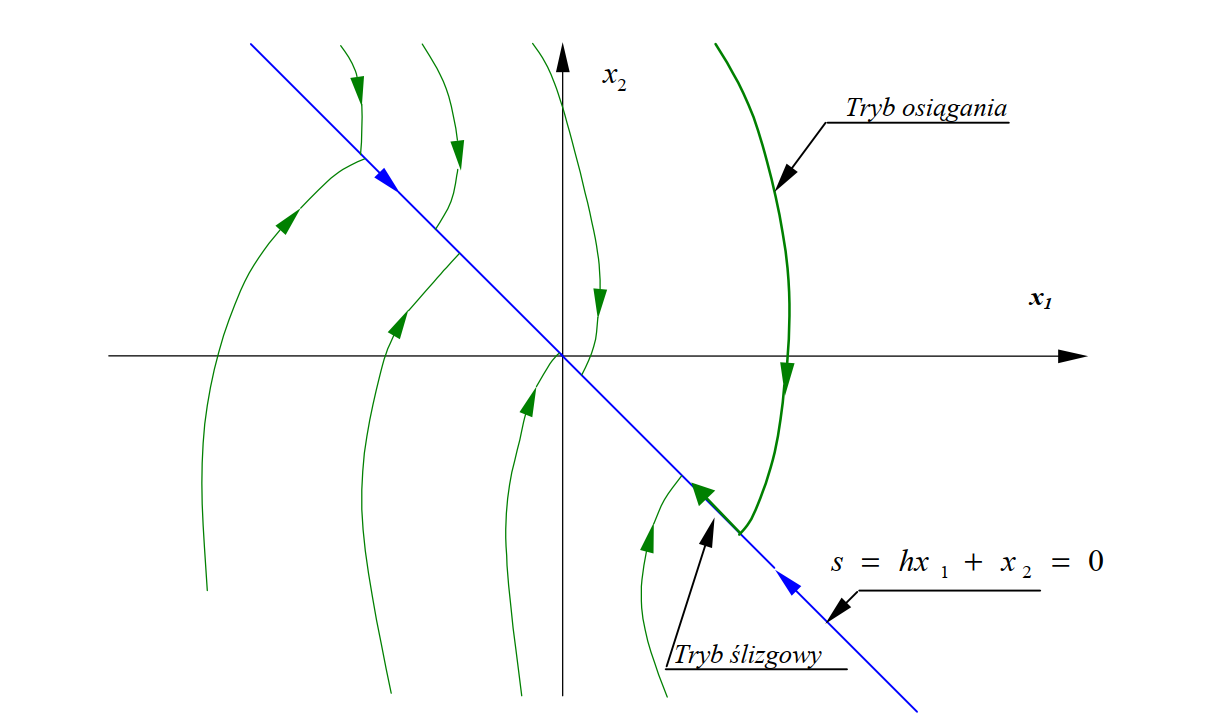
\includegraphics[width=1\linewidth]{figures/fig6_1}
  		\caption{Przyk?adowe trajektorie w przestrzeni zmiennych stanu uk?adu ze sterowaniem
  			?lizgowym, z wyr�?nieniem trybu osi?gania i trybu ?lizgowego.}\label{rys:6.1}
  	\end{center}
  \end{figure}
  %
  \section{Sterowanie predykcyjne mechanizm�w wielocz�onowych}
  \section{Sterowanie LQR/LQG mechanizm�w wielocz�onowych}
%-----
